\documentclass{thesisclass}
% Based on thesisclass.cls of Timo Rohrberg, 2009
% ----------------------------------------------------------------
% Thesis - Main document
% ----------------------------------------------------------------

%% -------------------------------
%% |   New Title Page Info       |
%% -------------------------------

% select your thesis type
\newcommand{\docType}{1} % Options: 0 = Bachelor Thesis, 1 = Master Thesis, 2 = Practical Report
\newcommand{\mainTitle}{Your Title}

\newcommand{\authorName}{Giulia Boccuccia}

\newcommand{\reviewerOneName}{Prof.\ Dr.-Ing.\ Samuel Kounev}
\newcommand{\reviewerOneTask}{First Reviewer}

% only required for Master's thesis
\newcommand{\reviewerTwoName}{Prof.\ Dr.\ Dummy} % Always use backslashes after abbreviation to prevent LaTeX from treating the period as the end of a sentence, which would otherwise add incosistent extra horizontal spacing
\newcommand{\reviewerTwoTask}{Second Reviewer}

\newcommand{\advisorOneName}{Name Advisor 1}
\newcommand{\advisorOneTask}{First Advisor}

% if only one advisor remove next two lines
\newcommand{\advisorTwoName}{Name Advisor 2}
\newcommand{\advisorTwoTask}{Second Advisor}

% if no external advisor remove next two lines
%\newcommand{\advisorExtName}{Name External Advisor}
%\newcommand{\advisorExtTask}{External Advisor}

\newcommand{\submissionTime}{XX. Month 20YY}

%% -------------------------------
%% |  Information for PDF file   |
%% -------------------------------
\hypersetup{
 pdfauthor={\authorName},
 pdftitle={\mainTitle},
 pdfsubject={\ifcase\docType Bachelor Thesis\or	Master Thesis\or Practical Report\fi},
 pdfkeywords={Not set}
}

%% -------------------------------
%% | Information for Declaration |
%% -------------------------------
\newcommand{\place}{Place}

%% ---------------------------------
%% | ToDo Marker - only for draft! |
%% ---------------------------------
% \todo{...} is provided by the todonotes package loaded in thesisclass.cls.
% To disable all todos for the final version, load the package with the
% "disable" option instead, e.g. \usepackage[disable]{todonotes}.
% \usepackage[disable]{todonotes}


%% --------------------------------
%% | Old Marker - only for draft! |
%% --------------------------------
% Remove this section for final version!
\newenvironment{deprecated}
{\begin{color}{gray}}
{\end{color}}


%% --------------------------------
%% | Settings for word separation |
%% --------------------------------
% Help for separation:
% In german package the following hints are additionally available:
% "- = Additional separation
% "| = Suppress ligation and possible separation (e.g. Schaf"|fell)
% "~ = Hyphenation without separation (e.g. bergauf und "~ab)
% "= = Hyphenation with separation before and after
% "" = Separation without a hyphenation (e.g. und/""oder)

% Describe separation hints here:
\hyphenation{
% Pro-to-koll-in-stan-zen
% Ma-na-ge-ment  Netz-werk-ele-men-ten
% Netz-werk Netz-werk-re-ser-vie-rung
% Netz-werk-adap-ter Fein-ju-stier-ung
% Da-ten-strom-spe-zi-fi-ka-tion Pa-ket-rumpf
% Kon-troll-in-stanz
}

% Make sure to include this before the begin of the document!
\DeclareAcronym{TBD}{
  short = TBD ,
  long  = To Be Done
}



%%%%%%%%%%%%%%%%%%%%%%%%%%%%%%%%%
%% Here, main documents begins %%
%%%%%%%%%%%%%%%%%%%%%%%%%%%%%%%%%
\begin{document}


% Choose language as required
\selectlanguage{english}
% \selectlanguage{ngerman}

\frontmatter
\pagenumbering{roman}
%!TEX root = thesis.tex

\begin{titlepage}

	\newgeometry{
		margin=0mm,
		noheadfoot,   % Removes space for header and footer
		nomarginpar   % Removes space for marginal notes
	}


	\begin{tikzpicture}[remember picture,overlay]
		%% Coordinates
		\coordinate (text_pos) at (55mm, 0);
		% Background Image
		\node [inner sep=0pt] (background_img) at (15, -17) {
\includegraphics[width=38cm]{logos/Marienberg_wuerzburg_verlauf.png}};
		% White Sidebar
		\node [fill=white, minimum width=82.6mm, minimum height=600mm] (box) at (current page.north west){};
		% White band for both university logos.
		\fill[white]
			([shift={(41.3mm,-42mm)}]current page.north west)
			rectangle ([shift={(0mm,-66mm)}]current page.north east);
		\node [anchor=west, inner sep=0pt] (uniwuelogo)
		at ([shift={(48mm,-54mm)}]current page.north west) {
			
\includegraphics[width=45mm]{logos/unilogo4cohne_mittel.jpg}
		};
		% The source PDF is a full page: crop its blank margins (in bp).
		\node [anchor=west, inner sep=0pt] (torvergatalogo)
		at ([shift={(110mm,-54mm)}]current page.north west) {
			\includegraphics[width=65mm,trim=14bp 747bp 376bp 0bp,clip]{logos/torvergata_logo.pdf}
		};

		%% ----- Titles -----
		% Doc Type
		\node [anchor=north west, inner sep=0pt, text width=170mm, align=flush left]
		at ([shift={(55mm,-20mm)}]current page.north west){
			\renewcommand{\baselinestretch}{1.5}
			\huge\textsf{\textcolor{titlecolor}{
					\ifcase\docType
						Bachelor Thesis\or
						Master Thesis\or
						Practical Report
					\fi
				}}
		};

		% Title
		\node [anchor=north west, inner sep=0pt, text width=130mm, align=flush left]
		at ([shift={(57mm,-70mm)}]current page.north west){
			\Huge\textsf{\textbf{\textcolor{titlecolor}{\mainTitle}}}
		};

		%% ----- Authors & Reviewers -----
		\node [anchor=north west, inner sep=0pt, text width=120mm, align=flush left]
		at ([shift={(55mm,-170mm)}]current page.north west) {
			\setlength{\parindent}{0pt}%
			\Large\textsf{\textcolor{titlecolor}{%
					% --- Author ---
					\textbf{\authorName} \\
					Matricola: \studentNumber \\[0.2cm]
					\homeUniversity\\
					\homeDepartment\\
					\degreeProgramme\\[0.5cm]
					\hostUniversity\\
					\authorDepartment\\
					\authorChair\\[1cm] % Spacing before supervisors
					%
					\ifnum\docType=2 % No Reviewers or advisors for practical report
					\else
						% --- Reviewer 1 ---
						\textbf{\reviewerOneName} \\
						\reviewerOneTask \\[\smallskipamount]
						%
						% --- Reviewer 2 ---
						\ifdefined\reviewerTwoName
							\textbf{\reviewerTwoName} \\
							\reviewerTwoTask \\[\smallskipamount]
						\fi
						%
						% --- Advisor 1 ---
						\textbf{\advisorOneName} \\
						\advisorOneTask \\[\smallskipamount]
						%
						% --- Advisor 2 ---
						\ifdefined\advisorTwoName
							\textbf{\advisorTwoName} \\
							\advisorTwoTask \\[\smallskipamount]
						\fi
						%
						% --- External Advisor ---
						\ifdefined\advisorExtName
							\textbf{\advisorExtName} \\
							\advisorExtTask
						\fi
					\fi
				}}%
			%% If more names are needed, just add them here like above. Be aware that there must not be an empty newline inside, so use % like above
		};




		%% ----- Footer -----
		% Date
		\node [anchor=north west, inner sep=0pt, text width=60mm, align=flush left]
		at ([shift={(57mm,-280mm)}]current page.north west){
			\Large\textsf{\textcolor{titlecolor}{\textbf{Submission\\}\submissionTime}}
		};

		\node [anchor=north west, inner sep=0pt, text width=110mm, align=flush left]
		at ([shift={(95mm,-285mm)}]current page.north west){
			\hfill\Large\textsf{\textcolor{titlecolor}{\textbf{\webadress}}}
		};

	\end{tikzpicture}

	\pagecolor{background}
\end{titlepage}
\restoregeometry

\pagecolor{white}
% \nopagecolor % If you have problems with a dark reader, try this option instead

\blankpage
\let\mainlang\languagename
\selectlanguage{english}
%!TEX root = ../thesis.tex

\chapter*{Abstract}
\dots



\selectlanguage{ngerman}
%!TEX root = ../thesis.tex
\chapter*{Zusammenfassung}
\dots



\selectlanguage{\mainlang}


%% -------------------
%% |   Directories   |
%% -------------------
% set the table of contents depth (= section levels which should be included in TOC)
\setcounter{tocdepth}{2}
\selectlanguage{english}
\tableofcontents
\blankpage


%% -----------------
%% |   Main part   |
%% -----------------
\mainmatter
\pagenumbering{arabic}
%!TEX root = ../thesis.tex
\chapter{\introduction}
\label{ch:introduction}

\ac{TBD}, \acp{TBD} (for plural)

To reference other sections, you can use \texttt{\textbackslash\{cref\}}. This is an improved version of the reference command that also prints the type (section, figure, \dots).

To reference online sources, be sure not to forget the \textit{urldate} field~\cite{google}.
% always use ~ before the cite command. This is a non-breaking space, so that there are no newlines in between the last word and the citation

You can also cite multiple sources~\cite{google,KiHeKo2014-LT-DLIM} together.

%!TEX root = ../thesis.tex
\chapter{\background}
\label{ch:background}
In this chapter,  we provide informations about various terms and concepts that are used in this thesis.
\begin{definition}
Definitions can be useful for technical/mathematical thesis. There are also other environments and also the proof environment. They are defined in \texttt{thesisclass.cls}. Have a look! You can also define your own ones if your supervisor is fine with it.
\end{definition}

\begin{lemma}\label{lem:just_a_lemma}
This is a lemma.
\end{lemma}

\begin{theorem}[Gödel's incompleteness theorem]
    This is a theorem and it also has a name.
\end{theorem}
\begin{proof}
    Theorems usually come with proofs.
    This one follows from \Cref{lem:just_a_lemma}.
\end{proof}


%!TEX root = ../thesis.tex
\chapter{\relatedwork}
\label{ch:relatedwork}

\cite{KiHeKo2014-LT-DLIM}

%!TEX root = ../thesis.tex
\chapter{\approach}
\label{ch:approach}

\section{Section A}
\label{sec:approach:section-a}

\begin{table}[h]
    \caption{This is an example table to be listed in List of Tables.}
    \label{tab:example}
    \centering
    \begin{tabular}{cc}
        \toprule
        Header Column 1 & Header Column 2 \\ 
        \midrule
        Data Point A    & $2^{128}$ iterations \\ 
        Data Point B    & AES-GCM \\ 
        \bottomrule
    \end{tabular} 
\end{table}

\section{Section B}
\label{sec:approach:section-b}


%!TEX root = ../thesis.tex
\chapter{\implementation}
\label{ch:implementation}

\begin{lstlisting}[language=erlang, frame=single, breaklines=true, numbers=left, caption={Hello World Program in Erlang.}]
-module(hello).
-export([hello_world/0]).

hello_world() -> io:fwrite("hello, world\n").
\end{lstlisting}

\begin{lstlisting}[language=cpp, frame=single, breaklines=true, numbers=left, caption={Program in C++.}]
#include <iostream>
int main() {
    std::cout << "Hello, World!" << std::endl;
    this->run();
    int a = 0;
    if (a <= 5){
        return 1;
    }
    // comment line
    return 0;
}
\end{lstlisting}

\begin{lstlisting}[language=yaml, frame=single, breaklines=true, numbers=left, caption={YAML Example}]
# A sample yaml file
key: value
array:
  - item1
  - item2:
        anotherKey: anotherValue
\end{lstlisting}

\newpage

\begin{lstlisting}[language=pseudo, frame=single, breaklines=true, numbers=left, caption={Pseudo Code Example}]
items = [1,2,3]
# Print each item in the list
for i in items:
    if i > 2:
        print("MyItem: "+i)
\end{lstlisting}



\begin{lstlisting}[language=docker, frame=single, breaklines=true, numbers=left, caption={Dockerfile Example}]
FROM python:3.13
WORKDIR /usr/local/app

# Install the application dependencies
COPY requirements.txt ./
RUN pip install --no-cache-dir -r requirements.txt

# Copy in the source code
COPY src ./src
EXPOSE 8080

# Setup an app user so the container doesn't run as the root user
RUN useradd app
USER app

CMD ["uvicorn", "app.main:app", "--host", "0.0.0.0", "--port", "8080"]
\end{lstlisting}

\newpage

\begin{lstlisting}[language=json, frame=single, breaklines=true, numbers=left, caption={JSON Example}]
{
    "key": "value",
    "pair": [
        "first": 0,
        "second": "null"
        # comment line
    ]
}
\end{lstlisting}

%!TEX root = ../thesis.tex
\chapter{Evaluation}
\label{ch:evaluation}


\section{Figures}
\begin{figure}[h]
	\centering
	
\includegraphics[width=0.6\linewidth]{logos/DescartesLogo_ohneSchatten_gross.png}
	\caption[Logo of the Descartes research group.]{Logo of the Descartes research group of the Chair of Software Engineering of University of Wuerzburg. This long story is not included in the list of figures because this is the long description of the image. The list of figures will only contain the text specified in the square brackets before this long description.}
	\label{fig:descarteslogo}
\end{figure}

\begin{figure}[h]
	\centering
	\begin{subfigure}[b]{0.3\textwidth}
		\centering
		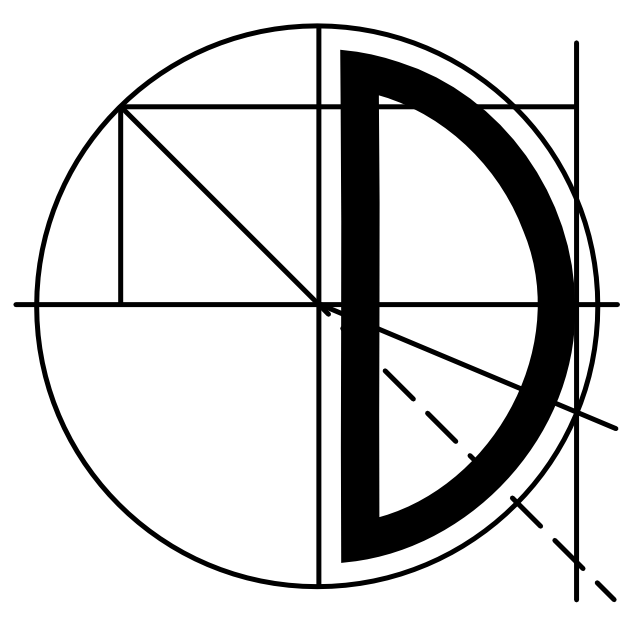
\includegraphics[width=\textwidth]{logos/DescartesSymbol_gross.png}
		\caption{Symbol placed on the left side.}
		\label{fig:descartessymbol1}
	\end{subfigure}
	\hfill
	\begin{subfigure}[b]{0.3\textwidth}
		\centering
		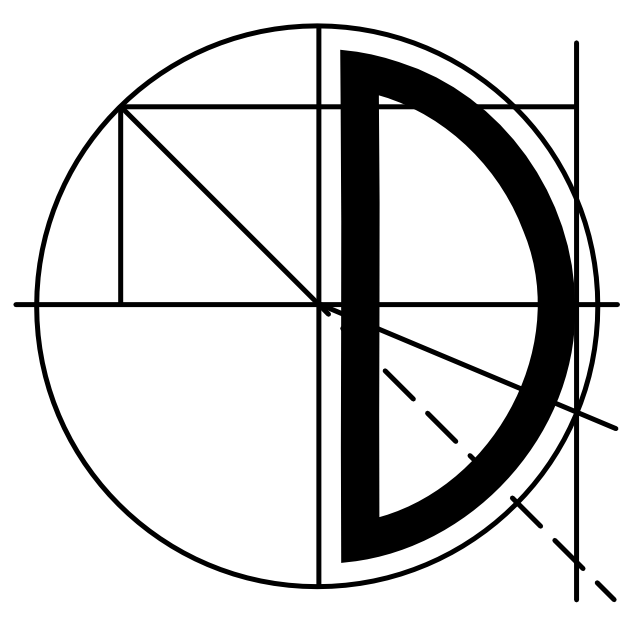
\includegraphics[width=\textwidth]{logos/DescartesSymbol_gross.png}
		\caption{Symbol placed in the middle.}
		\label{fig:descartessymbol2}
	\end{subfigure}
	\hfill
	\begin{subfigure}[b]{0.3\textwidth}
		\centering
		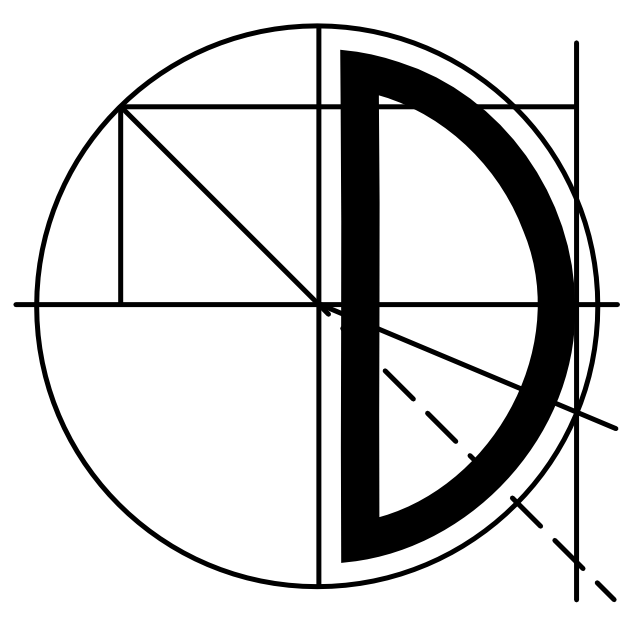
\includegraphics[width=\textwidth]{logos/DescartesSymbol_gross.png}
		\caption{Symbol placed on the right side.}
		\label{fig:descartessymbol3}
	\end{subfigure}
	\caption{Symbol of the Descartes research group.}
	\label{fig:descartessymbol}
\end{figure}

It is also possible to include \textit{.svg} figures via the \textit{svg} package, e.g.\ \verb|\includesvg{logos/example}|. This requires compiling with \verb|--shell-escape| and having \textit{Inkscape} installed locally. The resulting \textit{.pdf} is cached next to the source file.
\begin{figure}
%\includesvg{...}
\end{figure}


\section{Units}
To properly print units for measurements (e.g.\ time), use the \textit{siunitx} package.

Example: \qty{3}{\second} or \qty{8}{\milli\second} or \qty{222}{\kilo\metre\per\hour} or \qtyrange{10}{20}{\second} or \qty{10\pm 5}{\second}

Have a look at the \href{https://ctan.org/pkg/siunitx?lang=de}{package documentation} for more examples.

\section{ToDos}
Sometimes it may be worth, noting down a todo for later.\todo{This is a ToDo!}

You can later disable them by using \verb|\usepackage[disable]{todonotes}|.\todo{Don't forget to change that!}
However, you can also just delete them.

%!TEX root = ../thesis.tex
\chapter{\conclusion}
\label{ch:conclusion}



%% ----------------
%% |   Listings   |
%% ----------------

\cleardoublepage
\phantomsection
\addcontentsline{toc}{chapter}{\listfigurename}
\listoffigures

\cleardoublepage
\phantomsection
\addcontentsline{toc}{chapter}{\listtablename}
\listoftables

\cleardoublepage
\phantomsection
\addcontentsline{toc}{chapter}{\lstlistlistingname}
\lstlistoflistings



%% --------------------
%% |   Acronyms   |
%% --------------------
\printacronyms[
	name=\trans{Abkürzungsverzeichnis}{Acronyms},            % The title of the section
	heading=chapter*
	% display=all             Use this if all entries shall be printed regardless if they are used
]
\addcontentsline{toc}{chapter}{\trans{Abkürzungsverzeichnis}{Acronyms}}
\markboth{\trans{Abkürzungsverzeichnis}{Acronyms}}{\trans{Abkürzungsverzeichnis}{Acronyms}}

%% --------------------
%% |   Bibliography   |
%% --------------------
\cleardoublepage
\phantomsection
\addcontentsline{toc}{chapter}{\bibname}

\bibliographystyle{ieeetran_modified}

\bibliography{thesis}

%% ----------------
%% |   Appendix   |
%% ----------------
\cleardoublepage

%!TEX root = thesis.tex

% Hint: You can not reference the appendix as a whole, rather reference individual sections or figures inside the appendix.
\appendix

\section{First Appendix Section}
		\label{Anhang-Implementierung}
		
\setcounter{figure}{0}
		
\begin{figure} [ht]
  \centering
   ein Bild
  \caption{A figure}
  \label{fig:BPMNBeispiela}
\end{figure}


\dots





%% -------------------
%% |   Declaration   |
%% -------------------
\cleardoublepage
\todo{Dont forget the Versicherung zur Leistungserbringung, which is strictly required by the Pruefungsamt. Download and fill out the latest version from the Uni Wuerzburg Homepage (uni-wuerzburg.de). Go to Studium -> Pruefungsangelegenheiten -> Formulare -> Abschlussarbeiten / Hausarbeiten -> Versicherung zur Leistungserbringung. Maybe ask your supervisor for help.}


\end{document}
